\documentclass{article}

\usepackage[a4paper, total={6in, 8in}]{geometry}

\usepackage{amsmath}
\usepackage{amsfonts}
\usepackage{amssymb}
\usepackage[T1, T2A]{fontenc}
\usepackage[utf8]{inputenc}
\usepackage[english, russian]{babel}
\usepackage{graphics}
\usepackage{graphicx}

\geometry{
 a4paper,
 total={170mm,257mm},
 left=20mm,
 top=20mm,
 }

\author{Александр Валентинов}
\title{Лабораторная работа 3.4.5}

\begin{document}
   \subsection*{Работа 3.4.5}
   \section*{Петля гистерезиса (динамический метод)}
   
   \paragraph{Цель работы:} изучение петель гистерезиса ферромагнитных материалов с помощью осциллографа.
   
   \paragraph{В работе используются:} автотрансформатор, понижающий трансформатор, интегрирующая цепочка, амперметр, вольтметр, электронный осциллограф, делитель напряжения, тороидальные образцы с двумя обмотками.

   \subsubsection*{Схема установки}
   \begin{figure}[h]
   \centering
   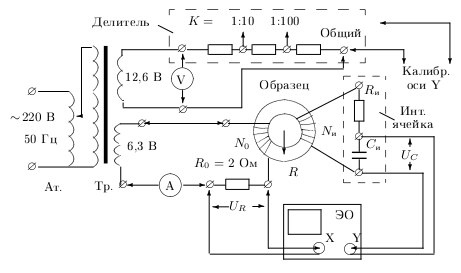
\includegraphics[width=10cm]{fig1.jpg} 
   \caption{Схема установки для исследования намагничивания образцов} 
   \label{fig.1} 
   \end{figure}

   \subsubsection*{Теория}
   
   Цена деления оси $X [\text{A/м}]$ осциллографа:
   \begin{equation}
      \label{e1}
      H = \frac{IN_0}{2\pi R}
   \end{equation}
   Цена деления оси $Y [\text{Тл}]$ осциллографа:
   \begin{equation}
      \label{e2}
      B = \frac{R_\text{и} C_\text{и} U_\text{вых}}{S N_\text{и}}
   \end{equation}
   Постоянная времени:
   \begin{equation}
      \label{e3}
      \tau = RC = \frac{U_\text{вх}}{\Omega U_\text{вых}}
   \end{equation}
   Дифференциальная магнитная проницаемость:
   \begin{equation}
      \label{e4}
      \mu_\text{дифф} = \frac{1}{\mu_0} \frac{dB}{dH}
   \end{equation}
   
   \subsection*{Исполнение}
   \paragraph{Феррит}
   \begin{flalign*}
   & K_x = 20 \text{ мВ} \quad K_y = 20 \text{ мВ} \quad I = 109 \text{ мА} &\\
   & S = 3.0 \text{ см}^2 \quad 2\pi R = 25 \text{ см} \quad &\\
   & N_0 = 35 \quad N_u = 400 &\\
   \end{flalign*}
   Цены деления осциллографа, рассчитанные по формулам \eqref{e1}, \eqref{e2}:
   \[
      c_H = 9.3 \text{ А/м} \quad c_B = 0.067 \text{ Тл}
   \]
   Коэрцитивная сила:
   \[
      H_c = (7 \pm 1) \text{ A/м}
   \]
   Индукция насыщения:
   \[
      B_s = 0.13 \pm 0.01 \text{ Тл}
   \]
   Дифференциальная магнитная индукция по формуле \eqref{e4} (см. графики):
   \[
      \mu_\text{дифф} = 2900 \pm 400
   \]

   \paragraph{Пермаллой}
   \begin{flalign*}
   & K_x = 20 \text{ мВ} \quad K_y = 1 \text{ В} \quad I = 139.6 \text{ мА} &\\
   & S = 3.8 \text{ см}^2 \quad 2\pi R = 24 \text{ см} \quad &\\
   & N_0 = 40 \quad N_u = 200 &\\
   & c_H = 11 \text{ А/м} \quad c_B = 0.52 \text{ Тл} &\\
   & H_c = 24 \pm 2 \text{ A/м} \quad B_s = 0.6 \pm 0.1 \text{ Тл} &\\
   & \mu_\text{дифф} = 64000 &\\
   \end{flalign*}

   \paragraph{Кремнистое железо}
   \begin{flalign*}
   & K_x = 50 \text{ мВ} \quad K_y = 50 \text{ мВ} \quad I = 356 \text{ мА} &\\
   & S = 1.2 \text{ см}^2 \quad 2\pi R = 10 \text{ см} \quad &\\
   & N_0 = 35 \quad N_u = 350 &\\
   & c_H = 58 \text{ А/м} \quad c_B = 0.48 \text{ Тл} &\\
   & H_c = 58 \pm 11 \text{ А/м} \quad B_s = 1.3 \pm 0.1 \text{ Тл} &\\
   & \mu_\text{дифф} = 125000 &\\
   \end{flalign*}

   \paragraph{Калибровка.} Осциллограф откалиброван верно, см. тетрадь.

   \paragraph{Постоянная времени.} Значения постоянной времени, рассчитаной по формуле
   \[
      \tau_0 = R_\text{и}C_\text{и} = 0.4 \text{с}
   \]
   и по формуле \eqref{e3} $\tau = 0.38$ совпадают.

   \[
      R = 20000 \text{Ом} \gg \frac{1}{\Omega C} = 1000 \text{Ом}
   \]

   \begin{table}[h!]
   \begin{center}
       \caption{Результаты эксперимента}
   \begin{tabular}{|*{4}{r|}}
   \hline 
                & Феррит  & Пермаллой     & Кремнистое железо \\ \hline 
     $H_c$, А/м & 7/8-600 & 24/4          & 58/8              \\ \hline 
     $B_s$, Тл  & 0.13/0.2-0.4 & 0.6/1.08 & 1.3/2.0           \\ \hline 
     $\mu_\text{дифф}$ & 2900  & 64000    & 125000            \\ \hline 
    \end{tabular} 
   \end{center}
   \end{table} 

   \begin{figure}[h]
   \centering
   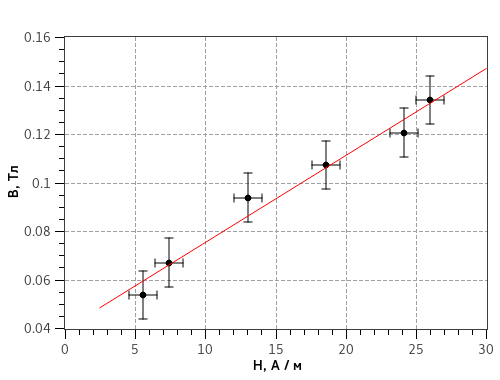
\includegraphics[height=6cm]{plot1.png} 
   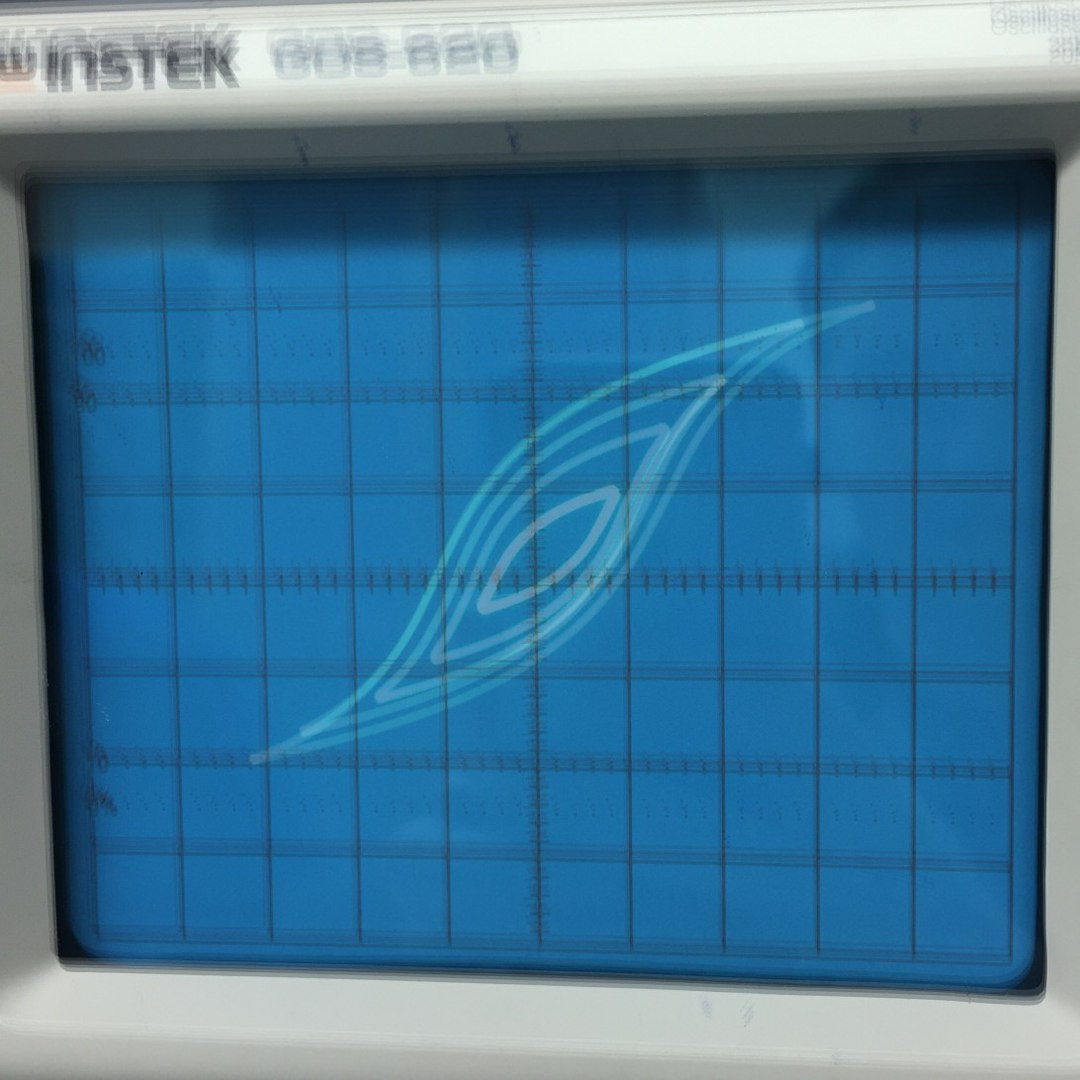
\includegraphics[height=6cm]{fig2.jpg}   
   \caption{Начальная кривая намагничивания для феррита} 
   \label{fig.2} 
   \end{figure}
       
   \begin{figure}[h]
   \centering
   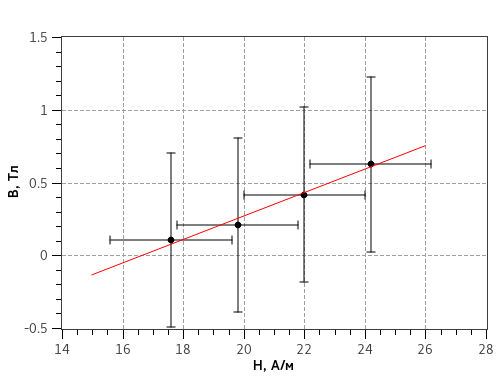
\includegraphics[height=6cm]{plot2.png} 
   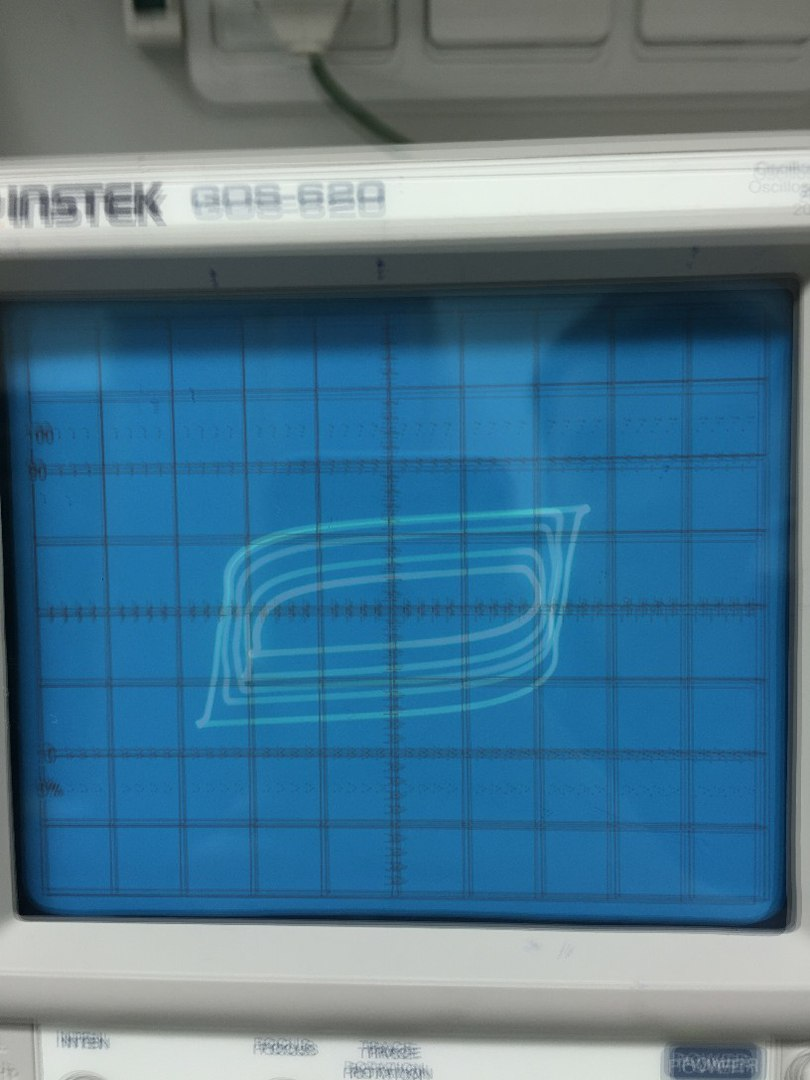
\includegraphics[height=6cm]{fig3.jpg}  
   \caption{Начальная кривая намагничивания для пермаллоя} 
   \label{fig.3} 
   \end{figure}

   \begin{figure}[h]
   \centering
   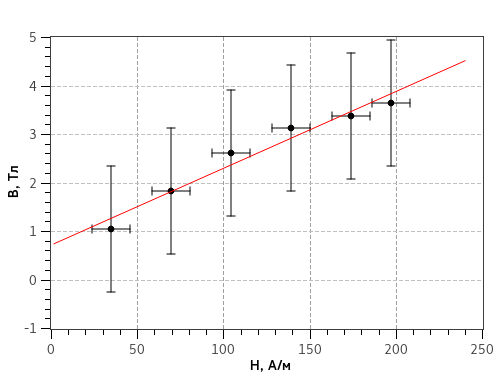
\includegraphics[height=6cm]{plot3.png} 
   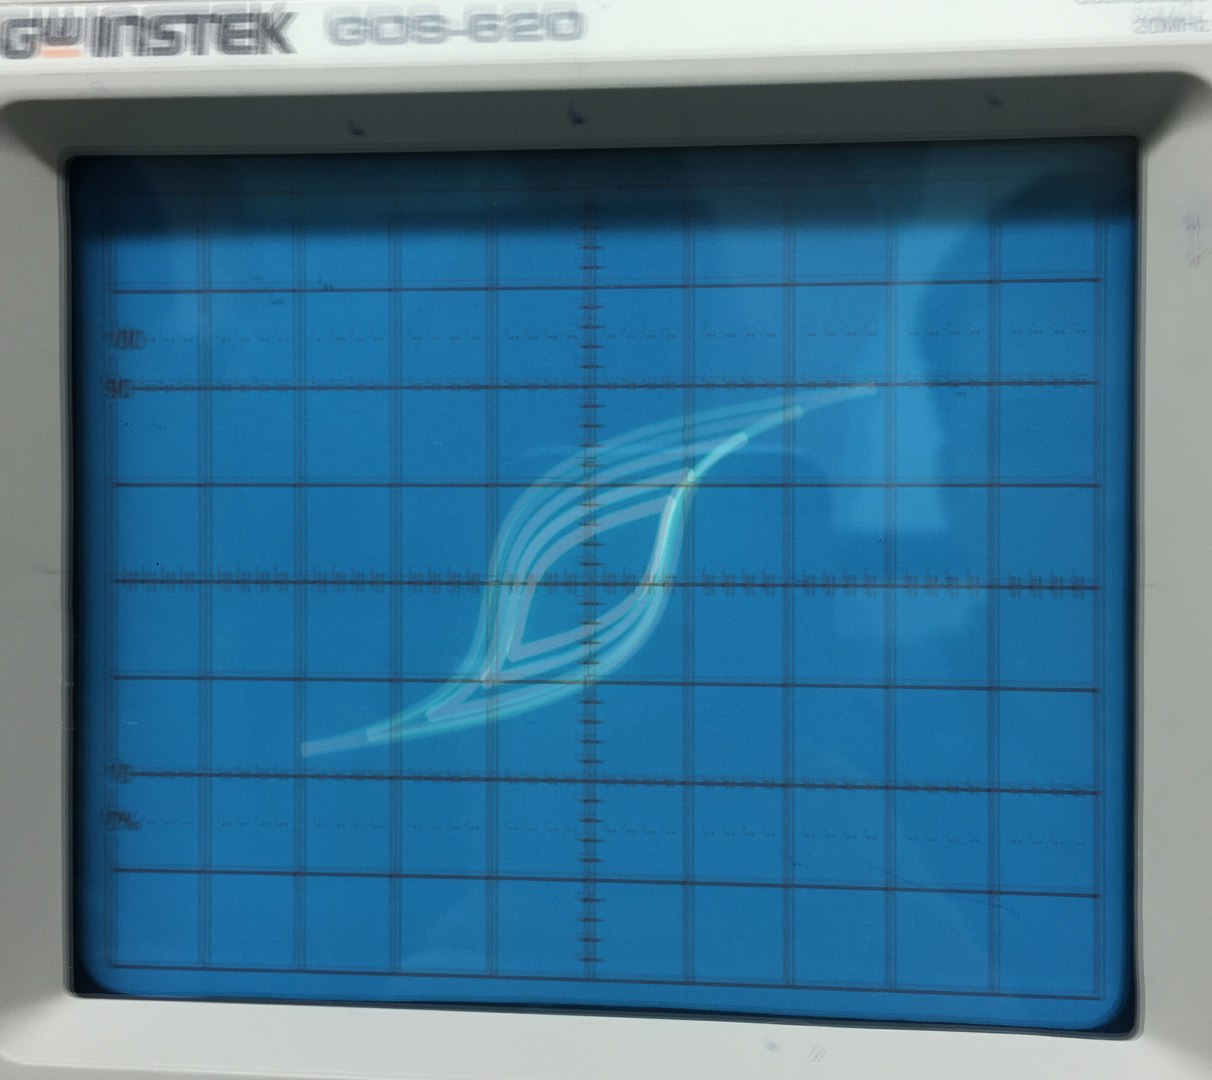
\includegraphics[height=6cm]{fig4.jpg}  
   \caption{Начальная кривая намагничивания для кремнистого железа} 
   \label{fig.4} 
   \end{figure}
\end{document}
